\documentclass[review]{elsarticle}

\usepackage[utf8]{inputenc}

\usepackage{lineno,hyperref}
\modulolinenumbers[5]

%% Necessary for multiple images in a row
\usepackage{graphicx}
\usepackage{caption}
\usepackage{subcaption}
\usepackage{booktabs} % for table* env.
\usepackage{multirow} % for row spanning

%% Para los colores de las anotaciones, eliminar para vf!!
\usepackage{color}
\usepackage{soul} % para tachar palabras
\setstcolor{teal}

\usepackage{float}

%% Commands for table format
%\newcolumntype{R}[2]{%
%    >{\adjustbox{angle=#1,lap=\width-(#2)}\bgroup}%
%    l%
%    <{\egroup}%
%}
\newcommand*\rot{\multicolumn{1}{R{90}{1em}}}%
\renewcommand{\arraystretch}{1.2} % Aumentar el espacio entre filas de una tabla
\newcommand{\ra}[1]{\renewcommand{\arraystretch}{#1}}

%% --------------------------- Old revision system -------------------------------
%% Change to final when definitive version of the paper will be generated.
%%\usepackage[draft, lang=spanish, mode=multiuser]{fixme}

%%\FXRegisterAuthor{kcmd}{kenv}{klyone}
%%\FXRegisterAuthor{jcmd}{jenv}{jda}
%%\FXRegisterAuthor{fcmd}{fenv}{felipetg}
%% --------------------------- Old revision system -------------------------------

%% Commands for the annotations
\usepackage[spanish, colorinlistoftodos, textsize=tiny]{todonotes}

%% Para los colores de las anotaciones, eliminar para vf!!
\usepackage{color}
\usepackage{soul} % para tachar palabras
\setstcolor{teal}

%% Standard notes
\newcommand{\ftglnote}[1]{\todo[bordercolor=violet, backgroundcolor=yellow]{#1}}
\newcommand{\klyonelnote}[1]{\todo[bordercolor=red, backgroundcolor=yellow]{#1}}
\newcommand{\ftgnote}[1]{\todo[bordercolor=violet, backgroundcolor=yellow, noline]{#1}}
\newcommand{\klyonenote}[1]{\todo[bordercolor=red, backgroundcolor=yellow, noline]{#1}}

%% Notes with high level of importance
\newcommand{\ftglwarning}[1]{\todo[bordercolor=violet, backgroundcolor=orange]{#1}}
\newcommand{\klyonelwarning}[1]{\todo[bordercolor=red, backgroundcolor=orange]{#1}}
\newcommand{\ftgwarning}[1]{\todo[bordercolor=violet, backgroundcolor=orange, noline]{#1}}
\newcommand{\klyonewarning}[1]{\todo[bordercolor=red, backgroundcolor=orange, noline]{#1}}

\journal{Journal of \LaTeX\ Templates}

%%%%%%%%%%%%%%%%%%%%%%%
%% Elsevier bibliography styles
%%%%%%%%%%%%%%%%%%%%%%%
%% To change the style, put a % in front of the second line of the current style and
%% remove the % from the second line of the style you would like to use.
%%%%%%%%%%%%%%%%%%%%%%%

%% Numbered
%\bibliographystyle{model1-num-names}

%% Numbered without titles
%\bibliographystyle{model1a-num-names}

%% Harvard
%\bibliographystyle{model2-names.bst}\biboptions{authoryear}

%% Vancouver numbered
%\usepackage{numcompress}\bibliographystyle{model3-num-names}

%% Vancouver name/year
%\usepackage{numcompress}\bibliographystyle{model4-names}\biboptions{authoryear}

%% APA style
%\bibliographystyle{model5-names}\biboptions{authoryear}

%% AMA style
%\usepackage{numcompress}\bibliographystyle{model6-num-names}

%% `Elsevier LaTeX' style
\bibliographystyle{elsarticle-num}
%%%%%%%%%%%%%%%%%%%%%%%

\begin{document}

\begin{frontmatter}

\title{A fully programmable White-Rabbit node for PPS distribution system of the SKA Telescope}
%\title{Elsevier \LaTeX\ template\tnoteref{mytitlenote}}
%\tnotetext[mytitlenote]{Fully documented templates are available in the elsarticle package on %\href{http://www.ctan.org/tex-archive/macros/latex/contrib/elsarticle}{CTAN}.}

%% Group authors per affiliation:
%\author{Elsevier\fnref{myfootnote}}
%\address{Radarweg 29, Amsterdam}
%\fntext[myfootnote]{Since 1880.}

%% Group authors per affiliation:
\author{Miguel Jiménez-López, Felipe Torres-González, Javier Díaz}
\address{CITIC, ETSIIT, University of Granada, Spain}

%% or include affiliations in footnotes:
%\author[mymainaddress,mysecondaryaddress]{Elsevier Inc}
%\ead[url]{www.elsevier.com}

%\author[mysecondaryaddress]{Global Customer 
%Service\corref{mycorrespondingauthor}}
\cortext[mycorrespondingauthor]{Corresponding author.}
\ead{klyone@ugr.es,felipetg@ugr.es,jda@ugr.es}

%\address[mymainaddress]{1600 John F Kennedy Boulevard, Philadelphia}
%\address[mysecondaryaddress]{360 Park Avenue South, New York}

%\listoffixmes

\begin{abstract} 
	This contribution is focused on finding a solution to provide a very 
	accurate PPS signal distribution for the international project known as 
	Square Kilometer Array (SKA) Telescope.The SKA will be the largest 
	radio-telescope of the world and it will be located in two different 
	geographical areas (South-Africa and Australia/New Zeland). 
    
    On each one of those locations, there will be placed hundred of antennas 
    whose individual observations will be combined as if they would be acquired 
    by only big one antenna. In order to archive that, a high level of 
    synchronization accuracy must be provided to each one of the antennas, more 
    precisely, it is consider a 2ns time requirement. That accuracy can't be 
    achieved by the current standard synchronization technologies, because of 
    that, we proposed a new design based on a FPGA-SoC device with an improved 
    version of the hardware clocking circuitry and the White 
    Rabbit (WR) protocol.
    
    In this context, 
	the WR Zynq Embedded Node (WR-ZEN) is the chosen platform to be used in the 
	SKA PPS distribution system. Our implementation is tested in different 
	scenarios in order to check that the system works in special conditions 
	varying the temperature. It is necessary because the SKA's deployment will 
	be performed in dessert zones and the environment is not as stable as a 
	laboratory. Finally, the conclusions extract from the present work justify 
	that the WR protocol seems to work properly with all the SKA's requirements 
	and compensates temperature change conditions. Finally, we present most 
	promising work lines and some tasks related to evolve the White Rabbit 
	technology for the SKA system in the future work section.
\end{abstract}

\begin{keyword}
	Square Kilometer Array, White Rabbit, Synchronization, Network, Gigabit Ethernet, Optical fibre, GNNS
\end{keyword}

\end{frontmatter}

\linenumbers

\section{Introduction}

The DAQ \cite{daq:book1} systems are responsible for converting the analog environment signals into digitial domain and send this data to a computer. Then, it can be processed to perform several tasks such as analysis, monitoring and control. Nowadays, there are many industrial \cite{daq:res} and scientific applications \cite{daq:sensor-networks} that require a DAQ system. However, these applications are normally composed of several nodes that are located at different places. The distributed DAQ systems must be implemented in these cases. These kind of systems need a computer network to allow data sharing between different nodes. The distributed DAQ systems also include a specific node that is responsible for receiving all data, process it and extract useful information about a certain event. It is important to note it is necessary to define some mechanisms in order to match data related with the same event coming from different nodes. One possible solution is to implement a synchronization mechanism in the distributed DAQ network sharing the time information between different nodes. Thanks to the synchronization, a event can be identified by the time it occurred.

%The DAQ systems have several sensors in different places to get environment information. A %computer network must be used in these system in order to ensure that all the data can be %shared. The main concern related to these system is the need to match information about the %same event in different nodes. 

There are many mechanisms to distribute time information and signals in distributed systems. Some of them use Global Navigation Satellite System (GNSS) receivers to get timing from Satellites (GPS, Glonass, Galileo) meanwhile others use wired protocols to provide the time reference 
through the network. The GPS approach is widely used in many systems that require accurate synchronization since various instrumentation can be easily connected to different GPS receivers. The main concern related to the GPS system is sensitive to jamming issues. However, some studies reveal that the synchronization mechanisms can help and reduce the negative effects related to the interferences \cite{NOURA2016130}. Alternatively and thanks to the packet networks popularity, the timing protocols are little by little imposing as main solution for time transfer over the network. Low performance protocols as NTP, the protocol used in Internet to synchronize the computers through the network), \cite{ntf:ntp_std} are widely used while for industrial applications the preferred protocol is the IEEE-1588v2 (known as PTPv2) \cite{ieee:ieee1588_std} \cite{itu:TG8275_1_Y_1369_1}. IEEE-1588v2 is an industrial evolution of NTP, characterized by the utilization of hardware time-stamping mechanisms that significantly improved time synchronization accuracy. Typically, NTP provides about 1 ms synchronization accuracy while PTPv2, working on very well designed time-aware networks is able to achieve about 50 ns synchronization accuracy. The IEEE-1588v2 is a candidate technology for control applications such as Smart Grid \cite{NAFI201623} where the time requirement are very strict and the synchronization is one of the key aspects to take into consideration \cite{COLAK2016396}.
In the synchronization framework, it is important to distinguish between frequency, phase and time distribution.

The first case regards to the distribution of the oscillator signal through a wire or to provide a mechanism to regenerate the clock frequency. This is usually  called syntonization. 
The phase distribution is normally implemented enconding phase information in a pulse that is transmitted every second through the wire. This mechanism is known as PPS signal and is used as a reference to identify when a new second starts.
The time distribution refers to the Coordinated Universal Time (UTC) /TAI (International Atomic Time) time information sharing between different elements in the network. It ensures that all the event are trigged at the same timing in the entire network. There are several packet-based (NTP, PTP, PTPv2) or serial protocols (NMEA) that are responsible for measuring the propagation time and exchange this information between nodes. 
A network is synchronized when takes into consideration these three elements: frequency, phase PPS) and time.

Some scientific facilities need a distributed DAQ system to perform its activity in the proper way. One example is the SKA \cite{ska:project_website} project. It is an international project to build a radio telescope tens of times more sensitive and hundreds of times faster at mapping the sky than today's best radio astronomy facilities. It will become the world's largest radio telescope. The SKA telescope is composed of several types of antennas to be sperad over long distances so a distributed DAQ system is needed for data sharing and synchronization. Once completed, it will generate data at a rate more than 10 times today’s global Internet traffic. The SKA will be used to answer fundamental questions of science and about the laws of nature and imposes a technological challenge never faced before.

In the case of SKA, different solutions for time transfer were analyzed. For instance, GPS devices provide a reference frequency (10-50 MHz), a PPS signal and a serial code to provide the time (typically based on the NMEA protocol). The standard packet-based protocols such as NTP, PTP or PTPv2 are not appropiated to fulfill the SKA's strict timing specifications (2 ns for the SKA Telescope).
In this context, out research group at the University of Granada is working as a partner in the Signal and Data Transport (SaDT) \cite{ska:sadt_website} work package. Our proposal consits on the development of a new device based on the technology called WR \cite{ohwr:wr_wiki} to disseminate a PPS signal very accurately over fibre links. WR is an evolution of IEEE-1588v2 protocol and able to distribute an absolute time reference with an accuracy of 1 ns. Equipment located at each endpoint delivers a PPS signal with its edge aligned to the start of the UTC second. Therefore, each telescope can then be phased up by observing the white light fringe on one or more bright, compact sources.

This paper is organized in several sections. The current one 
presents the introduction and the motivation. Section \ref{sec:ska} introduces the SKA Telescope project, the different network and timing requirements that evidence that industrial solutions are not suitable for SKA. Section \ref{sec:wr} focuses on the fundamentals of the WR technology. Section \ref{sec:ska-pps-system} describes the proposed end-node for SKA including the justification, architecture and software support. The synchronization performance of the proposed solution is evaluated in different scenarios with special consideration on the scalability of the WR technology for the SKA deployment and the synchronization accuracy taking into account different meteorological conditions in section \ref{sec:experiments}. Final remarks and conclusions are described in section \ref{sec:conclusion}. Last sections(\ref{sec:future-work} and \ref{sec:acknowledgments}) are described the future work and the acknowledgments.

%\textcolor{red}{La motivación es pobre. Hay que ser más preciso: qué necesita SKA, qué es lo %que no cubren otras tecnologías similares (o qué desventajas tienen) y cómo (hemos %pensado)/pensamos solucionarlo.}

%\textcolor{red}{la siguiente sección debería ser el Related Work}


\section{The SKA telescope} \label{sec:ska}

The Square Kilometer Array (SKA) will be the largest radio-telescope of the world. Located in two different geographical areas (South-Africa and Australia/New Zeland) it will be one of the great physics machines of 21st Century and, when complete, one of the world’s engineering marvels. It will be constructed on different phases SKA1 (phase 1 2018-2023) and SKA2 (phase 2 2023-2033). The development will be deployed using on two different pathfinders existing on each place (MeerKAT in South Africa and ASKAP in Australia). 

The key science goals for this instrument are:

\begin{itemize}
	\item {Formation of the 1st galaxies in a dark Universe dominated by atomic gas.}
	\item {Evolution of the atomic gas till the current epoch.}
	\item {Strong Field Tests of Gravity Using Pulsars and Black Holes.}
	\item {Acceleration in the expansion of the Universe not understood yet.}
	\item {Habitable extra-solar planets (proto-planetary disks, biomarkers).}
\end{itemize}

The SKA facility will use several kind of antennas targeting different geographical locations and time schedule. During SKA1 and according to the SKA1 System Baseline description \cite{ska:baseline_description_v2}, for building such facility two different kinds of antennas will be used according to their capabilities to sense. They are: 

\begin{itemize}
	\item {SKA-LOW, 50 - 350 MHz Australia, 131,000 aperture array dipole 512 stations of 256 antennas.}
	\item {DISHES, 350 MHz - 14GHz South-Africa SKA1\_Mid 350 MHz – 14 GHz 64 MeerKAT dishes plus additional 133 SKA1 dishes.}
\end{itemize}

\begin{figure}[h]
	\includegraphics[scale=0.25]{img/ska_instruments}
	\caption{The SKA's low frequency (right) and the mid-frequency (left) instruments.  SKA Telescope will be built on two different phases. These images (adapted from \cite{ska:multimedia_rsrcs}) illustrate key numbers corresponding to SKA1 phase (starting 2018). }
	\label{fig:ska_instruments1}
\end{figure}

The SKA1 telescope is being designed to optimize its performance and some key facts about both types of instruments are shown on Fig. \ref{fig:ska_instruments1}. 

The scale of the SKA Telescope represents a huge leap forward in both engineering, research and development towards building and delivering a unique instrument, with the detailed design and preparation now well under way. The unprecedented high performance specifications requires the utilization of best technologies and design strategies possible and represent an unprecedented challenge for all the elements to be built. 

\subsection{SKA Telescope Network}

The SKA Telescope use different types of networks to guarantee a proper operation of the infrastructure. The design of the network corresponds to the Signal and Data Transport (SaDT) element \cite{ska:sadt_website} and it includes all hardware and software necessary for the transmission of data and information between the Elements of the SKA. SADT also contains details about the provision of timing which is critical for interferometry.
The data network includes the Digital Data Backhaul (DDBH) that transports signals from the radio telescopes to the Central Signal Processor (CSP), and data products from the CSP to the Science Data Processor (SDP) and from the SDP to the regional SKA Data Centers. The total data rates are very high, approximately 80 Tb/s for the DDBH links and another 80Tb/s for the CSP links. 
Also covered by the SaDT is the Monitor and Control (M\&C) that transmits and receives monitoring and control information throughout the system and includes the Telescope Manager, itself comprised of three logical networks: Production Network, Engineering Network and Safety Network, the Network Manager as well as local monitoring and control.

The final part of the SaDT is the Synchronization and Timing (SAT) that provides frequency and clock signals from a central clock ensemble to all elements of the system to maintain phase information to the required accuracy for all receptors, and timing signals for data identification and time critical activities at the receptors, and the CSP and SDP. To maintain phase coherence across the array requires short-term timing \ftglnote{¿Esto no debe ir en singular?}precisions of around 1 ps, while for the requirements for the long-term timing for pulsar require 10 ns accuracies over 10 year periods. The timing is critical to the functionality of the SKA to work as a unified large telescope using a technique known as interferometry. This contribution will focus on the high accuracy synchronization method used for SKA1 responsible to provide a PPS (Pulse Per Second) signal to the critical elements. 

\begin{figure}[h]
	\includegraphics[scale=0.4]{img/ska_network_arch}
	\caption{The SKA Telescope network architecture is composed by three networks: the data network (red), the M\&C network (green) and the SAT network (blue). An external clock reference, UTC traceable, is provided to the whole Telescope elements in order of providing an unique time reference.}
	\label{fig:ska_net_arch1}
\end{figure}

\klyonelnote{This figure must be re-made because it is not ours. It would be convenient to use the same terminology than figure's caption...}

\subsection{Distribution of high accuracy timing signals for ska1}

As determined by SaDT, SKA telescope should be able to distribute a commune frequency reference to all the telescopes and, in addition, provide a uniform time reference to register all the events with ultra-high accuracy through time stamps. This task is done by the SAT (Synchronization and Timing) element that belongs to SaDT. The SKA timescale is maintained by the central clock ensemble for each telescope and will be steered to within designed limits of UTC (Coordinated Universal Time) and monitored with respect to UTC via GNSS time transfer techniques. These clock ensembles form the fundamental timescale for SKA and will be the basis for precision measurements of pulsars and other time-dependent phenomena. As consequence, during this distribution, UTC refers to UTC (SKA), as realized by the central SKA clock ensemble.
This article will focus on the solutions to distribute the UTC time by means of PPS (Pulse-Per-Second signal). This PPS signal guarantees that all the scientific data are time-tag using a common reference. This time reference has high requirements coming from science that are not mandatory by other elements of the SKA systems as the monitor and control network. For these other elements, standard time transfer protocols as NTP or IEEE-1588 are a feasible solution. For the Telescope core, we illustrate that the high performance requirements imposed by the challenging scientific goals force to provide much more sophisticated solutions. 
The PPS distribution system will be in charge to deliver its output at the following locations:

\begin{itemize}
	\item {Each of the 133 dishes of SKA1-MID, and once to the Meerkat system. The maximum receptor baseline lengths are between 120-150 km.}
	\item {The core of SKA1-LOW, and the 45 stations in total along the 3 spiral arms. The maximum receptor baseline lengths are between 70-80 km. }
	\item {The encoded absolute time signal will be delivered to each of the three CSPs.}
\end{itemize}
 
Note that if the offset frequency scheme is to be applied to all SKA1-Mid dishes, an additional 64 STFR endpoints will be needed in SKA1-mid. This provides between 182 and 246 endpoints to synchronize. 
The general array SAT requirements for the frequency distribution is 1 ps while the time synchronization and time-stamp requirement is 10ns. SaDT uses different mechanisms for achieving goals, frequency dissemination and PPS distribution. As consequence, because the goal in this contribution is just describing a solution for PPS distribution, the contribution work only considers the second requirement, the 10 ns synchronization as needed for example for the long-term timing Pulsar studies. Note that a complete description of the SKA network elements and topology is out of the scope of this contribution and only the requirements needed is presented to properly understand the need of the solution here developed. 
It is important to remark than the 10 ns requirement is the \ftglnote{Quizás sería interesante explicar el término time-budget}time-budget allocated for the whole network. Because elements such as main clock also consume part of this budget, it translates into PPS-distribution time requirement of 5 ns. The error here includes PPS distribution, delay center precision, Dish timing transport and time-stamping errors. This time-budget should be distributed on the different elements of the system that rely on the network topology that determine the number of hops. Based on current SAT network topology, the target specification for the elements of the PPS distribution system provides them an average time-budget better than 2 ns. This is a quite challenging goal not only because impose a high accuracy synchronization goal but especially having into account the installation environmental conditions. The SKA1 use aerial optical fiber networks that are significantly affected by the large temperature excursion during operation, more than 50º due to the installation on desert locations of Sud-Africa and Australia. Furthermore the outdoor wind velocities during normal operation could achieve up to 40 km/h. it makes the fibers oscillate, changing their length, which must be compensated on real-time during execution or averaged them out. 
Next section will provide the description of the solution proposed to be use on SKA1 as mechanism for PPS distribution. 


\section{The White Rabbit synchronization protocol}

In the case of SKA, different solutions for time transfer were analyzed. For instance, GPS devices provide a reference frequency (10-50 MHz), a PPS signal and a serial code to provide the time (typically based on the NMEA protocol). \textcolor{red}{This approach is widely used in many systems that require accurate synchronization (since various instrumentation can be easily connected to different GPS receivers) but it is sensitive to jamming issues. However, some studies reveal that the synchronization mechanisms can help and reduce the issues related to the interferences \cite{NOURA2016130}.  Alternatively and thanks to the packet networks popularity, the timing protocols are little by little imposing as main solution for time transfer over the network. Low performance protocols as Network Time Protocol (NTP), the protocol used in Internet to synchronize the computers through the network), \cite{ntf:ntp_std} are widely used while for industrial applications the preferred protocol is the IEEE-1588v2 (known as Precision Time Protocol or PTPv2) \cite{ieee:ieee1588_std} \cite{itu:TG8275_1_Y_1369_1}. IEEE-1588v2 is an industrial evolution of NTP, characterized by the utilization of hardware time-stamping mechanisms that significantly improved time synchronization accuracy. Typically, NTP provides about 1 ms synchronization accuracy while PTPv2, working on very well designed time-aware networks is able to achieve about 50 ns synchronization accuracy. The IEEE-1588v2 is a candidate technology for control applications such as Smart Grid \cite{NAFI201623} where the time requirement are very strict and the synchronization is one of the key aspects to take into consideration \cite{COLAK2016396}.
Although previous approaches are quite accurate, they are not appropriated to fulfill the specifications of the 2 ns requirement associated to the SKA telescope. As alternative solution, the utilization of the White Rabbit (WR) protocol has been proposed because it is an evolution of IEEE-1588v2 protocol and able to distribute an absolute time reference with an accuracy of 1ns. Equipment located at each endpoint delivers a 1PPS signal with its edge aligned to the start of the UTC second. Therefore, each telescope can then be phased up by observing the white light fringe on one or more bright, compact sources. (\textbf{esto precisamente me parece más cosa de introducción/motivación})}

The White Rabbit \gutinote{una vez puesto el acrónimo, solo se usa el acrónimo} (WR) technology is an international, collaborative project started at CERN in 2009, and then joined by other laboratories and companies. It was born as replacement technology for the timing system at CERN, but thanks to its versatility, improved performance, compared to the alternatives, and open nature of the project, it was quickly adopted by other scientific institutions. There is also a strong interest in private companies to extend WR in the industrial world such as Seven Solutions \cite{sevensols:wr}. Furthermore, from its very early stages, WR was launched as an open Sw/Hw initiative with sources available at the Open Hardware Repository \cite{ohwr:repo}. This encouraged different companies and research institutions to openly collaborate in its development.

The WR protocol extends Precise Time Protocol version 2 (PTPv2) with extra messages, proposed to be included in the new PTP release (PTPv3) as High Accuracy profile \textcolor{red}{[REF]}
. Its main goal is to provide a synchronization accuracy better than 1 ns and precision in the scale of picoseconds. The major improvements introduced in the WR protocol address weak aspects of the PTPv2: the limitation in the phase difference measurements to one period of the system clock; and the assumption of symmetry between the transmission and reception paths. It inherently performs self-calibration over optical fiber links and it is capable of distributing time to a very large number of devices with very small degradation. Nevertheless, this technology in the origin was not designed to address large distances or provide embedded nodes with monitoring and dependable mechanism. Although SKA is working on improving both issues, we particularly focus on this contribution on providing a novel platform capable disseminate the PPS signal ad with flexibility and dependability characteristics.  

%\textst{WR is based on other technologies such as the L1 synthonization of Synchronous Ethernet (SyncE), an extension of PTPv2 (WR-PTP) and additional phase %alignment techniques. The L1 synthonization is responsible for transmitting the master clock inside the data stream in order to slave devices can recover it from %the network and adjust their oscillator frequencies to follow the reference clock.} 

%\textsterling{WR also uses additional phase alignment techniques as the Digital Dual Mixed Time Difference (DDMTD) that is a module responsible for measuring the %phase between two clocks. This information is used to change the frequency of the local oscillator for the synchronization process.}

The WR synchronization mechanisms include the following elements:

\begin{itemize}
	\item {Frequency synchronization (syntonization): It uses L1 syntonization \gutinote{yo diría physical layer L1, y ya en el resto del paper diría solo L1}
	of Synchronous Ethernet (SyncE) to encode the clock signal in the data 
	carrier. It is responsible for recovering the clock from the network and to 
	adjust local oscillator to follow it.}
	\item {Phase synchronization: The physical clock of a node is retransmitted to the master element and viceversa so that master can compare the phase of this signal (coming from the slave) with its own phase. The deviation should be equal to the propagation time of the signal through the fiber. The master can determine the phase difference between its own clock and the network recovered one and send back this information to the slave. The phase measurement is performed by an IP core known as Digital Dual Mixed Time Difference (DDMTD) present in the gateware design.}
	\item {Time synchronization: It is implemented by PTPv2 protocol and provides a global notion of time to the entire network. WR also takes into account the asymmetries in the propagation time due to the utilization of different wavelengths in the same fiber link improving the accuracy of standard PTP protocol.}
\end{itemize}

%%Internal oscillators of the WR devices run locked to the master's reference clock of the network, allowing precise phase difference 
%%measurements between the master clock and the slave clock. 

WR implements mechanisms to ensure deterministic and reliable data transfer 
between a thousand of nodes connected with  optical fiber links up to 10 km. 
However, it can easily be extended up to 50 km without significant degradation 
and up to 120 km without the needs of optical amplification. 

\subsection{Network topology and devices} \label{subsec:wr-net-devices}
A typical WR 
network is arranged in tree topology. This is very common in timing networks 
where time reference is propagated down-link from a root device, known as Grandmaster, that can be connected to a very stable clock, such as an atomic clock 
or a GPS receiver \textcolor{red}{[REF]}. Currently, new network topologies are under-study in WR to 
add some mechanisms to improve fault tolerance \gutinote{la redundancia mejora la tolerancia a fallos, es decir, no puedes "mejorar" la redundancia, mejoras la tolerance a fallos desarrollando mecanismos de redundancia} and security. An example of 
this research is \cite{jlgutierrez-paper-redundancy} that incorporates the 
Transparent Clocks (TC) to WR protocol and allows implementing redundancy 
protocols such as HSR or PRP to ensure the data delivery and reception in 
critical applications.

The intermediate levels of the network disseminate the timing packets to the final 
nodes, which are composed of other devices such as WR Switches, WR-ZEN or WR-LEN 
that have several ports and can behave as PTPv2 Boundary Clocks (BC). Their 
different ports are divided into two types: one of them is the slave (up-link) 
and connects to the upper layer and the other ports are masters (down-links) 
and they are charged to propagate the synchronization to the next level of the 
hierarchy . The nodes of the last level of the network are known as Slave 
devices that recover the clock signal of the link and synchronizes their local 
oscillators to provide synchronization for a specific application or facility.
\textcolor{red}{[reescribirlo recortando un poco las frases, deberiais usar más la adjetivación en lugar de "and" and "and"]}
\textcolor{red}{[os tenéis que asegurar de referenciar en el texto las figuras, y utilizarlas de apoyo para explicar las cosas en el texto]}
\textcolor{red}{no son dos tipos de puerto, maestro-esclavo es un modelo de comunicación. Los puertos esclavos son "upstream" y los maestros "downstream"}
\textcolor{red}{hay que mantener cierta coherencia con mayúsculas y minúsculas. Si vais a poner Slave o slave, debéis mantenerlo a lo largo del texto}



\begin{figure}[H]
	\centering
	\includegraphics[scale=0.4]{img/wr_hierarchy}
	\caption{The WR network is a tree hierarchy where the root node is the Grand Master that is responsible for distributing the reference time signals. The intermediate elements are WR Switches that acts as Gigabit Ethernet switchers and as Boundary clocks propagating the time signals from the upper layers of the network. Finally, \textcolor{red}{the leaf nodes are known as nodes (esto es obvio, sobra)} which main purpose is to provide timing to another specific application.}
	\label{fig:wr_hierarchy}
\end{figure}



%\missingfigure{Añadir figura para mostrar la topología WR}

WR is designed to be fitted in a Field Programmable Gate Array (FPGA) device due to its flexibility to use in designs in a continuous development state. The source code is mainly written in Hardware Description Languages (HDLs) such as VHDL or Verilog. Moreover, there are several platforms that can implement WR that ensures the vendor-independent feature of WR. The most extended vendor in WR world is Xilinx, some examples of devices using Xilinx's FPGAs are the SPEC board \cite{ohwr:spec} and the WRS \cite{ohwr:wrs}. The other vendor used in WR is Altera. Some examples of boards could be found in \cite{cesar-altera-wr}. The main Intellectual Property (IP) block is the WR PTP core (WRPC) for WR nodes and the Real Time Subsystem (RTS) for WR switches. 

The utilization of the previous WR-compliant nodes in the SKA system presents an important problem: they are based on PCIe interface cards to be plugged on standard computers, microTCA or VME-64 crates and therefore, a specific computer is necessary to provide the high 
level software management functionalities. Although most of these cards can be used on stand-alone operation mode, they just use a FPGA device as processing engine and this make very complicated to add new functionalities or standard software tools. The main WR node designs include a soft-microprocessor on the FPGA gateware but it is not 
enough to fully solve the problem because it requires using complex 
non-standard firmware programming tools and it normally translates on high time-intensive development effort and makes difficult the upgrade of the system firmware. We have worked with these platform in order to build a sensor network based on the SPEC board allowing the PC-hosted and the standalone modes \cite{migueljl-paper-wr-spec}.

As a different solution, we present a new platform based on an enhanced technology: The WR Zynq Embedded Node (WR-ZEN) \cite{sevensols:wr_zen}. It is a new generation board that includes a Xilinx Zynq System-on-Chip (SoC) \cite{xilinx:zynq}. The Zynq SoC is composed of a FPGA and a hard ARM dual core microprocessor that can run an application that controls the hardware directly or a standard Operating System such as Linux that can host many different kind of processes at the same time. Moreover, the WR-ZEN allows developing gateware and software on the same chip, tightly integrating performance and flexibility thanks to the use of the co-design strategies. The WR-ZEN offers several advantages over the old WR-compliant nodes (WR-LEN, SPEC or SVEC) such as an enhanced standalone mode with a Linux system that can include high level software capabilities without an external PC and the new clocking circuitry among others. Accordingly, the WR-ZEN has been proposed to be used in the SKA project to implement the PPS distribution system and currently, it is being evaluated as a candidate solution for the SKA PPS distribution system.  

Next sections will present the proposed system for SKA and the main WR contributions: WR Precision Time Protocol for clock propagation and the generation of PPS signal. 


\section{The PPS distribution system for SKA}

The WR protocol requires a network topology similar to the ITU-T
G.8275.1/Y.1369.1 standard, a IEEE-1588v2 telecommunication profile that
describes a time-aware network capable to provide full timing support
\cite{itu:TG8275_1_Y_1369_1} as explained in previous section. It uses a master
time reference (SKA1 clock) that is distributed following a tree topology in a
master-slave configuration. The SKA PPS distribution system is composed of two
different kinds of devices:

\begin{itemize} \item {The WR Switches \cite{sevensols:wr_switch}. They are
			standard 1U height rack-mounted equipment with 18 SFP
			ports and are placed in the CSPs at each of the clock
			ensembles. For SKA1-MID, one is placed halfway along
			each of the 3 spiral arms to regenerate the signal for
		the longest links.} \item{The end-nodes. They consist of a
			WR-ZEN node \cite{sevensols:wr_zen} powered by a Zynq
			FPGA-SoC and placed on inside a 1U rack enclosure. They
			will be located at the cores of SKA1-LOW and
SKA1-SURVEY, along their spiral arms, one for each SKA1-MID dish and one for
each CSP.} \end{itemize}

The WR switches are responsible for generating the WR timing signal from the
SAT clock ensembles. They lock to an external 10MHz reference and to a PPS
signal, and use NTP or IRIG-B to determine the UTC time of each PPS edge.
Synchronisation between WR devices is performed over a a single fibre link up
to 120 km using commercial SFPs.  However, the distances for SKA1-MID are
longer and it is necessary to use intermediate WR switches as repeaters with a
penalty over the system performance due to increment of the inherent noise of
each WR device that it is propagated to the downstream nodes. An analysis of
the jitter evolution for network with many hops could be read in
\cite{torres2016scalability}. Thanks to network similarities between WR and
SKA, both can use the same single fibre strand available for the SAT network. 

\begin{figure}[H] \centering \includegraphics[scale=0.4]{img/ska_pps_network}
\caption{Network topology for PPS signal distribution based on WR switches and
nodes. The figure shows the different elements and the network topology. }
\label{fig:ska_pps_dist_network} \end{figure}

An important feature of the system to take into account is that the PPS pulse
itself at each station is derived from the reference frequency distributed from
the SKA clock and not from the WR system. In normal operations, the WR system
only monitors the absolute time of each PPS and reports it back activating an
alert if the PPS signal does not align with the start of the UTC second. This
condition indicates something is wrong in the timing chain and the station must
be discard data to avoid system data corruption. Other functionality associated
with the WR part is to temporarily alter the division ratio to bring the PPS
edge back in alignment with UTC time. In this case, fringe finding must then be
performed to restore full calibration again.

The centrally located WR switches and the WR end-nodes are connected to by a
single strand of single-mode fibre with LC/PC connectors and industry standard
bi-directional SFPs that use two wavelengths (downstream and upstream) to
produce optical signals to be transmitted. Finally the end nodes generate a PPS
signal available. 

As previously described, this solution requires WR switches and nodes. The
former are well-defined equipment with known interfaces and software support. 

For the implementation of the SKA nodes, we have proposed the utilisation of
the WR-ZEN board. Thanks to this new platform, the utilisation of a host
computer/crate to host the FPGA card can be avoided which reduces significantly
the equipment price and is also a remarkable improvement in term of
dependability which is a key factor taking into account that SKA Telescope
should have an annual availability of about 95\% of the time (although degraded
operation modes can be allowed under some circumstances).  Finally note that
all these features are possible keeping the full flexibility of a complete
CPU+FPGA system on a single board. 

In the following section we describe the proposed node hardware, gateware and
firmware that have been developed as a candidate solution for the SKA Telescope
PPS distribution system. 

\subsection{A PPS distribution node architecture}
\label{subsec:ska-pps-system-arch}

The PPS distribution system for SKA is based on the WR-ZEN platform that
provides the WR support in order to ensure the synchronisation accuracy in the
system. The first design of the PPS system includes the Fine Delay FMC card
that is used to generate the timing signals through mezzanine channels.
Moreover, it has two Network Interface Cores (NIC) that allows accessing
optical fibre ports as conventional Linux network interfaces. An introduction
to this platform is presented in \cite{migueljl-paper-wr-zen-intro} and a
contribution that improves the NIC bandwidth of the design in
\cite{jorgesg-paper-wr-zen-dma}. In addition, the WR-ZEN is also under study
for other FMC cards such as the FMC ADC one to build a distributed oscilloscope
\cite{joselj-paper-wr-zen-adc}.

Nowadays, the utilisation of the Fine Delay FMC card is still under discussion
and there is a possible design whose its final architecture could be addressed
without this module.

\subsubsection{Hardware} \label{subsec:hardware}

The WR-ZEN board is a proprietary design of the Seven Solutions company
developed in 2015. The major design changes respect to previous designs for
WR-nodes are the inclusion of a Zynq FPGA-SoC platform from Xilinx, and a
flexible and enhanced clocking scheme. The former, enables a more structured
design where the software can be organised in abstraction layers. This is
achieved by the inclusion of an Linux-like OS and many low-level drivers and a
Hardware Abstraction Layer (HAL). These components allow an easy and quick
development of new functionalities on top of all the software that interfaces
with the underlying hardware. A deeper detailing of the software structure is
given at subsection \ref{subsec:software}. The new clocking circuitry, makes
the new board suitable for many synchronisation applications with diverse
requirements.

\begin{figure}[H] \centering
	\includegraphics[width=0.7\linewidth]{img/wrzenv3_scaled}
	\caption[WR-ZEN board picture]{The picture shows the WR-ZEN board with
	the FMC Fine Delay connected. Main connectors are shown: Ethernet
	ports, SFP ports and the SMA connectors for the RF input/output
signals.} \label{fig:wrzen} \end{figure}

The FPGA-SoC platform breaks up design in two different parts: (i) the
Programmable Logic (PL) including modules described in HDL; and (ii) the
Processing System (PS) formed by all the software executed by the ARM
processor.  The inclusion of a hard-processor is something new in the node
architecture.  These problems have been solved by the WR-ZEN design: a powerful
hard-processor for software and more free resources in the FPGA side due to
pass some of the software from the embedded-processor to the ARM. In addition
to that, the Zynq platform includes the needed physical components by the WR
design: internal programmable PLLs, Gigabit Transceiver Ports (GTPs), and other
not strictly fundamental for a WR-node but which could be very helpful in
future designs such as Ethernet interfaces with hardware timestamping support
(allowing PTPv2 support). I/O ports are also very important because they will
interface with external components which can obtain synchronisation from the
base board. The most relevant I/O interfaces of the WR-ZEN are the FMC HPC
socket (support for the OHWR \cite{ohwr:repo} FMC cards
\cite{ohwr:fmc-fine-delay}), two SFPs sockets capable of BC configurations, and
many external RF connectors for input/output of RF signals and the PPS.

\begin{figure} \centering
	\includegraphics[width=0.7\linewidth]{img/zenclkschema} \caption[WR-ZEN
	clocking schema]{The figure depicts the new clocking schema presented
	in the WR-ZEN design. The most relevant changes considering previous
	designs are: the inclusion of an external PLL to lock an external
	stable clock reference (GM mode), and a flexible path in the main
	clocks path allowing the final user to choose between a low-noise PLL
	and a full-featured PLL with many options such as programmable output
delays.} \label{fig:zenclkschema} \end{figure}

The extended WR clock schema is depicted in Figure \ref{fig:zenclkschema}.
Besides including new components, the WR-ZEN design, upgrades some of them
looking for an increment of the clock stability. All the clock path: Digital to
Analogue Converter (DAC), Voltage-controlled crystal oscillator (VCXO),
Phase-Locked loop (PLL) has received an upgrade. A new DAC with a better
response time and stability, and low-noise VCXO and PLL have been included. But
the PLL from previous designs is maintained because it offers some key aspects
such as programmable output delays. To avoid cascading many PLLs, the signal
from the crystal oscillator (XO) is droved to the low-noise PLL first because
it allows bypassing its reference to other components without adding noise to
the reference. This schema enables using both PLLs at the same time. One of
them is used to generate all the WR-clocks and the other could be used to
generate custom frequencies. The WR general performance is limited by the noise
when locking to an external reference, in the so called Granmaster mode,
described in \cite{Rizzi2016}. The conclusion of that contribution is that in
order to decrease the noise when locking to an external reference, internal
PLLs in the FPGA should be avoid. Instead of it, it is recommended an Analogue
external PLL which locks to the external reference and generated the needed
clock signals by the internal elements of the WR-logic in the FPGA. That
enhanced features are included in the version 3.0 of the WR-ZEN as shown in
Figure \ref{fig:zenclkschema} looking to achieve the expected PPS distribution
stability requirements of the SKA project.


\subsubsection{Gateware} \label{subsec:gateware}

The gateware (FPGA firmware) is responsible for configuring the embedded ARM
microprocessor and the FPGA inside the Zynq SoC. The main block diagram is
shown in the Figure \ref{fig:gateware_first_level}. It includes the WRPC Dual
port (WRPC-2p) core that implements the high accuracy timing protocol based on
WR and provides basic capabilities such as Gigabit networking, timestamp
mechanism, debug interfaces, etc. The Gigabit transceiver (GT) ports include
needed modules to send/receive packets to/from the network. The Network
interface cores (NIC) are in charge of processing the incoming/outcoming
packets and notify these events to the ARM. The transmission time stamp unit
(TxTSU) is an additional module that allows recovering the outcoming packet
timestamps. The Fine Delay core controls the operation of the Fine Delay FMC
card if any is plugged into the FMC socket. The Wishbone (WB) Crossbar
interconnects all the elements of the architecture and eases the configuration
process performed by the ARM. The AXI-WB Bridge is a bus converter between AMBA
AXI and Wishbone ones. This conversion is needed because the ARM microprocessor
uses the AMBA specification while others components are based on WB.

\begin{figure}[H] \centering
	\includegraphics[scale=0.4]{img/gateware_first_level} \caption{Gateware
	project design. The figure shows the main components of the design. The
	most important one is the WRPC-2p core that is responsible for
	implementing the WR protocol. The GT ports allows to transmit/receive
	packets to/from the network through the optical SFP modules. The NIC
	cores manage Ethernet packets and behave as standard network interface
	cards for the ARM microprocessor. The AXI-WB Bridge translates AXI
	transactions into WB ones. It is important because the ARM is connected
	using AMBA specification meanwhile the WR FPGA cores use Wishbone bus
	standard. Finally, the Fine Delay core contains the needed resources to
control the Fine Delay FMC card.} \label{fig:gateware_first_level} \end{figure}

\subsubsection{Firmware} \label{subsec:firmware}

The firmware code is related to all the required functionalities by the WR
protocol. In the node architecture, the embedded software part of the WR
protocol and some device drivers runs in the soft-microprocessor described in
the previous section. The main tasks of the WR routines are the servo loop
algorithm which, maintains the lock to the recovered frequency from the master
device, and the implementation of the WR-PTP stack. In addition, a simple
Command Language Interface (CLI) is introduced to allow the user interaction
when it is used in standalone mode without an external PC.

\subsubsection{Software} \label{subsec:software}

The WR-ZEN is the first WR node taking advantage of a Linux based operative
system (OS) in a standalone configuration. Due to the inclusion of a dual-core
ARM microprocessor in the platform, the system design is not longer tied to
low-level software design. New functionalities, such as communication
protocols, management tools, etc., are quickly added thanks to the support
provided by the OS. The hardware abstraction layer and drivers help to abstract
the management of the underlaying logic. This middleware adds also more
security controlling the access to the hardware.

The software components are presented in the Figure
\ref{fig:software_architecture}.  It is divided into the userspace utilities
and the kernel support.  The former include the Zen library that implements the
basic functionalities for the Zen tools through the C standard library. The Zen
tools provides some mechanisms to program the FPGA design and connect to the
internal UART for debugging/configuration tasks among others.  Moreover, other
utilities are included to control the Fine Delay FMC card if it is plugged into
the FMC socket.

In the kernel side, some drivers have been implemented. The main one is the
\textit{zen} driver that is responsible for setting up all the IP cores in the
FPGA and creates the standard Linux network interfaces. The \textit{fmc} and
\textit{zio} drivers are retrieved from the OHWR repository and implements a
generic support for FMC and ZIO buses respectively.  The \textit{zio} driver
has been modified in order to work properly in the WR-ZEN platform.  The
\textit{zen-nic} kernel module is in charge of enabling/desabling the network
capabilities of the \textif{zen} driver. The \textit{fmc-fine-del} driver
provides basic functionalities for the Fine Delay FMC card.

As previously mentioned, there are dependencies between the different kernel
drivers and it establishes the installation order. The \textit{zen} one depends
on \textit{fmc}. The \textit{fmc-fine-del} needs \textit{zen}, \textit{zio} and
\textit{fmc}. The \textit{zen-nic} only uses the \textit{zen}.

\begin{figure}[H] \centering
	\includegraphics[scale=0.4]{img/software_architecture}
	\caption{Software architecture. The figure shows the software
	architecture used by the design. It is based on Linux kernel and
	several tools and drivers have been developed for the WR-ZEN board. The
	tools can be used to program the FPGA, update the soft-microprocessor
	code or connect to the virtual UART interface of the WRPC-2p. They call
	the Zen Library procedures that finally use C Library functions and
	switch to kernel mode through system calls. In the kernel space, the
drivers are responsible for implementing all the requested functionalities. }
\label{fig:software_architecture} \end{figure}

The next section describes the main performed experiments and the obtained
results.



\section{Experiments}

%% Section to describe and comment the results from the experiments performed.
%% lang: en-GB

In this section we detail the accomplished experiments and their results in 
order to evaluate the presented PPS distribution system for the SKA's timing 
system. The first experiment is a general characterization of the PPS 
distribution system. The second one emulates a example of WR network like the 
one needed to distribute timing in the SKA telescope, and evaluates the 
synchronization accuracy. Finally, the influence of external conditions over 
the fibre links and its effect on the synchronization accuracy is analysed.

The principal equipment and tools utilized during the experiments is listed 
below:

\begin{itemize}
    \item Two White Rabbit Switches to emulate a two-hops WR network. Both are 
    hardware version 3.4 and are flashed with the last version of the WR 
    firmware (v5.0).
    
    \item Two White Rabbit ZEN Time Provider (WR-ZEN TP) to test the 
    performance of the new developed platform as WR nodes of the SKA 
    facilities. Firmware version is 1.2 while the hardware is v3.0.
    
    \item A High-resolution counter from Keysight, the 52320A.
    
    \item Multiple components for the setup of the equipment:
    \begin{itemize}
        \item Small form-factor pluggable transceptors (SFPs) to establish the 
        link between WR devices. For the shorter links we've used the most 
        common bidirectional SFPs for WR: AXCEN 1310/1490 nm. For larger links, 
        we tried 
        SFPs from FiberStore: GE-BX-80 1490/1550 nm.
        \item Simplex optical fibre links (G652D). For the device 
        characterization short distance fibres have been used, meanwhile for 
        the scalability and temperature tests we have used long distance links: 
        20 and 50 km respectively.
        \item A OCXO Morion MV89 as frequency reference for the GM mode.
    \end{itemize}
    
\end{itemize}

\subsection{PPS performance of the WR-ZEN platform}
\label{subsec: charact_zen}

With this first experimental results we present a performance analysis of the 
PPS distribution using the WR-ZEN. The connection schema is formed by two 
WR-ZENs, one as WR master and the other as WR slave, whose PPS output signals 
are introduced in a time counter to measure the offset between them. With this 
experiment we focus on the WR-ZEN performance, so that we set all the equipment 
to a constant temperature and we use a short fibre link (few meters) in order 
to avoid instability occasioned by chromatic dispersion on long fibre links.

\begin{table*}\centering
	\ra{0.8}
	\begin{tabular}{@{} rccc@{}}%\toprule
		\textbf{$\tau$ (s)} & MDEV & TDEV (s)  & MTIE (s) \\ \midrule
		\small{1}     & 2.41e-11 & 1.39e-11  & 8.78e-11 \\
		%%\small{2}     & 8.18381977e-12 & 9.44986109e-12  & 9.27734375e-11 \\
		%%\small{4}     & 2.92095805e-12 & 6.74566367e-12  & 1.02539063e-10 \\
		\small{8}     & 1.05e-12 & 4.86e-12  & 1.02e-10 \\
		%%\small{16}    & 3.70004736e-13 & 3.41795734e-12  & 1.02539063e-10 \\
		%%\small{32}    & 1.36916757e-13 & 2.52956566e-12  & 1.02539063e-10 \\
		\small{64}    & 5.26e-14 & 1.94e-12  & 1.02e-10 \\
		%%\small{128}   & 2.41679947e-14 & 1.78603498e-12  & 1.02539063e-10 \\
		\small{256}   & 1.14e-14 & 1.69e-12  & 1.22e-10 \\
		\small{512}   & 6.76e-15 & 2.00e-12  & 1.22e-10 \\
		%%\small{1024}  & 4.60374214e-15 & 2.72176309e-12  & 1.22070312e-10 \\
		%%\small{2028}  & 3.37370493e-15 & 3.98911375e-12  & 1.22070312e-10 \\
		\small{4096}  & 1.20e-15 & 2.84e-12  & 1.31e-10 \\
		%%\small{8192}  & 8.69742436e-16 & 4.11358028e-12  & 1.56250000e-10 \\
		%%\small{16384} & 			   &                 & 1.66015625e-10 \\
		%%\small{32768} &				   &                 & 1.66015625e-10 \\
		
		\bottomrule
	\end{tabular}
	\caption{In this table it can be checked out the most relevant statistics 
	for the device characterization performed in the subsection \ref{subsec: 
	charact_zen}.}
	\label{tab:exp1res}
\end{table*}

The numerical results are included in Table \ref{tab:exp1res} and are 
represented graphically on Figures \ref{fig:mdev_exp1}, 
\ref{fig:tdev_exp1} and \ref{fig:mtie_exp1}. The slope of the Modified Allan 
Deviation curve shows that noise is dominated by white phase modulated noise. 
In the time domain, TDEV shows that the expected error is tens of ps and the 
worst-case showed in the MTIE plot is bounded around 200 ps for the sampling 
period. 

\begin{figure}
	\centering
	\begin{subfigure}[t]{0.48\textwidth}
		\includegraphics[width=\textwidth]{img/mdev_exp1}
		\caption[MDEV plot for the WR-ZEN]{Modified Allan Deviation plot for a 
		time transfer between two WR-ZEN.}
		\label{fig:mdev_exp1}
	\end{subfigure}
	~ % This symbol adds a white space between images
	\begin{subfigure}[t]{0.48\textwidth}
		\includegraphics[width=\textwidth]{img/tdev_exp1}
		\caption[TDEV plot for the WR-ZEN]{Time Deviation plot for a time 
		transfer between two WR-ZEN.}
		\label{fig:tdev_exp1}
	\end{subfigure}
\end{figure}

\begin{figure}
		\centering
		\includegraphics[width=0.5\textwidth]{img/MTIE_exp1}
		\caption[MTIE plot for the WR-ZEN]{Maximum Time Interval Error for a 
		time transfer between two WR-ZEN.}
		\label{fig:mtie_exp1}

\end{figure}

The obtained values reveal that the proposed WR node for the PPS distribution 
solution fulfils the requirements to be used in the SKA PPS distribution 
system. Although, it is necessary to evaluate it in more realistic conditions 
before concluding its goodness:

\begin{itemize}
	\item Evaluate the WR-ZEN as final node of a WR network. The purpose of 
	this device is to be placed on each acquisition instrument to provide an 
	accurate time reference. The results presented in the subsection 
	\ref{subsec: net_exp} states performance for a realistic WR deployment.
	
	\item Moreover, SKA facilities will be placed in a desert zone, and 
	the nodes will be linked by long-distance fibre links. Because of that, 
	it's 
	necessary to analyse if the meteorological conditions can degrade 
	significantly the synchronization accuracy. A thermal characterization of 
	the influence of the variation of propagation delays in the PPS accuracy is 
	presented in subsection \ref{subsec:temp}.
\end{itemize}   

\subsection{WR scalability for SKA} %% Buscar un nombre mejor
\label{subsec: net_exp}

The next experiment covers a scalability analysis of the WR solution for the 
SKA timing system. In section \ref{sec:ska} there is a estimation of the final 
nodes that need to be synchronized for the SKA: around 250 endpoints that 
must be synchronized with an accuracy below 2ns. A WR network with only two 
hops is suitable to synchronize up to 306 end-nodes by the use of WR Switches as 
Boundary Clocks.

We set up a test network composed by a WRS at the top, which is locked to an 
external time reference, another WRS as intermediate BC and a WR-ZEN as 
endpoint. This configuration allows synchronizing up to 306 WR nodes with an 
expected performance similar to the results obtained in our test for the WR-ZEN.

\begin{figure}
	\centering
	\includegraphics[width=0.7\linewidth]{img/prueba_red}
	\caption[WR Scalability test's setup for SKA]{To evaluate the scalability 
	of the WR solution for the expected SKA timing network, a sample WR 
	network has been evaluated. At the top there's a WRS as GM, a second layer 
	of WRS to finally provide synchronization to the end-nodes (WR-ZEN).}
	\label{fig:pruebared}
\end{figure}


All the equipment for that test was under laboratory conditions. To connect 
each one of the WR devices we've used a 20km fibre spool and SFPs from 
FiberStore (SFP-GE-BX80 with 1490/1550 nm wavelengths). PPS phase difference is 
measured from the WR-ZEN to the WRS in GM configuration using a Keysight 52320A 
counter along 4 hours.

\begin{figure}
	\centering
	\includegraphics[width=0.5\linewidth]{img/tdev_exp3}
	\caption[TDEV of the end-nodes in the scalability test.]{Time Deviation 
	plot comparing the PPS signal from the end-nodes (WR-ZEN) to the Grand 
	Master of the network.}
	\label{fig:tdevnet}
\end{figure}

TDEV and MTIE values have been calculated by octaves, the numerical 
values can 
be found in Table \ref{tab:netresults}. Graphical representations are included 
in Figures \ref{fig:tdevnet} and \ref{fig:mtienet} respectively. TDEV results 
show that expected synchronization accuracy for the end-nodes is around tens of 
ps. The maximum PPS error during this test is bounded in hundred of ps, which 
is more than enough what SKA needs (2ns).

\begin{table*}\centering
	\ra{0.8}
	\begin{tabular}{@{} rcc@{}}%\toprule
		& TDEV (s)  & MTIE (s) \\ \midrule
		\textbf{$\tau$ (s)}\\
		\small{1}     & 2.32e-11  & 1.36e-10 \\
		%\small{2}     & 1.33315382e-11  & 1.36718750e-10 \\
		%\small{4}     & 9.08699704e-12  & 1.36718750e-10 \\
		\small{8}     & 6.51e-12  & 1.36e-10 \\
		%\small{16}    & 4.48330572e-12  & 1.36718750e-10 \\
		%\small{32}    & 3.22792513e-12  & 1.36718750e-10 \\
		\small{64}    & 2.37e-12  & 1.46e-10 \\
		%\small{128}   & 2.02186966e-12  & 1.46484375e-10 \\
		%\small{256}   & 2.36616321e-12  & 1.46484375e-10 \\
		\small{512}   & 4.38e-12  & 1.61e-10 \\
		\small{1024}  & 7.27e-12  & 1.66e-10 \\
		\small{2048}  & 9.75e-12  & 1.75e-10 \\
		\small{4096}  & 7.97e-12  & 1.90e-10 \\
		%\small{8192}  &                 & 2.00195313e-10 \\
		
		\bottomrule
	\end{tabular}
	\caption{This table contains the Time Deviation and Maximum Time Interval 
	Error results from the scalability test.}
	\label{tab:netresults}
\end{table*}

With those findings, it's proved that a WR network with two levels can provide 
synchronization to all the equipment expected for the SKA facilities. 
Although long-distance fibre links have been used for that test, thermal 
influence should be take into account in order to confirm the goodness of the 
WR solution in the SKA timing distribution. The next experiment will evaluate 
how the temperature change in the fibre link can affect the accuracy of the 
synchronization. 


\begin{figure}
	\centering
	\includegraphics[width=0.5\linewidth]{img/MTIE_exp3}
	\caption[MTIE of the end-nodes in the scalability test.]{Maximum Time 
	Interval Error
	plot comparing the PPS signal from the end-nodes (WR-ZEN) to the Grand 
	Master of the network.}
	\label{fig:mtienet}
\end{figure}

\subsection{Fibre operational temperature influence on time accuracy}
\label{subsec:temp}

One of the key aspects of the timing solution for the SKA facilities is the 
influence evaluation of the external elements in the timing performance. 
Synchronization signals are spread over hundred of nodes which are connected by 
long distance fibre links. Meteorological elements, such as wind or large 
temperature changes, can alter propagation delays over the fibre 
links. The timing solution must compensate appropriately those effects in order 
to maintain the synchronization performance inside the limits required by the 
SKA's infrastructure.

On this contribution, we've focused on the temperature change effect over the 
cable
\textit{round-trip} time (CRTT) and the PPS performance. To evaluate that, we 
own a climate chamber in the laboratory and some fibre spools of tens of 
kilometers. 
We couldn't evaluate properly wind impact with our equipment, because of this, 
the experiments will only determine temperature effect on synchronization.

Theoretically, WR is able to dynamically calibrate the master to slave 
propagation delay from the total \textit{round-trip} time, and therefore PPS 
offset shall maintain constant even when the propagation delay changes. The 
accurate estimation of the one-way propagation delay is achieved by the use of 
a constant value, $\alpha$, which express the ratio between propagation times 
with the two wavelengths used in the WR link. A complete explanation of the 
link model could be read in \cite{Wlostowski2011} and \cite{Daniluk2012}.

In the real world, $\alpha$ is temperature dependent, because of the change in 
the refraction index due to a temperature variation in the fibre. For small and 
mid-distance links, in laboratory conditions, $\alpha$ is nearly negligible and 
the current link model behaves very well. The WR network in SKA will be formed 
by long distance links exposed to external elements. In the concrete situation 
of the South Africa facilities, the chosen location was the Karoo region. 
This region is a semi-desert area, very adequate to reduce human interferences 
in the high resolution data acquisition equipment, but with a inconvenient 
respect to the temperature point of view: desert zones have a high difference 
between day and night temperatures.

\begin{figure}
	\centering
	\includegraphics[width=0.7\linewidth]{img/tempsetup}
	\caption[Configuration of the climate chamber experiments]{Experimental 
		setup to analyse the influence of the temperature gradient over the 
		fibre link and the synchronization accuracy.}
	\label{fig:tempsetup}
\end{figure}

We performed a series of experiments introducing a 50 km length fibre spool in 
a climate chamber. The CRTT and the PPS offset between master and slave have 
been measured for a temperature range from 20 ºC to 50 ºC with 10 ºC steps. 
The average temperature difference between day and night in the Karoo region on 
each month is below 20 ºC, so the experiment covers comfortably the expected 
temperature operation conditions.

\begin{table*}\centering
	\ra{0.8}
	\begin{tabular}{@{} cccccc@{}}%\toprule
		& \multicolumn{2}{c}{\bfseries{RTT (ps)}} & &
		\multicolumn{2}{c}{\bfseries{PPS $offset_{SM}$ (ps)}} \\
		\cmidrule(l){2-3}  \cmidrule{5-6}
		\textbf{Spool temp (ºC)} & $\overline{x}$ & $s$ & & $\overline{x}$ 
		& $s$ \\ \midrule
		\small{20} & 478471695 & 303 & & 193 & 17 \\
		\small{30} & 478503719 & 50  & & 203 & 17 \\
		\small{40} & 478533492 & 807 & & 150 & 17 \\
		\small{50} & 478567050 & 399 & & 110 & 14 \\
		\bottomrule
	\end{tabular}
	\caption{Results of the thermal characterization for an operational fibre 
		temperature in range 20ºC to 50ºC with 10ºC steps.}
	\label{tab:temp}
\end{table*}

Our test is intended to prove the hypothesis that PPS offset is not related to 
the cable \textit{round-trip} time, i.e. changes in CRTT will not affect the 
synchronization accuracy. We have performed a series of experiments where the 
operational temperature of a 50 km fibre link is set in a point from 20ºC to 
50ºC. When the fibre reached the target temperature, we started to measure the 
rest of dependent values such as CRTT and PPS offset. All the WR equipment was 
calibrated in order to compensate the characteristic delays of each device 
following the official calibration procedure \cite{man:calib}.  The test setup 
is depicted in figure \ref{fig:tempsetup}.

The most relevant results are included in Table \ref{tab:temp}: (i) the mean 
value of CRTT and PPS offset samples, and (ii) their sample standard deviation. 
A total of 7200 samples (2 hours) per temperature step have been used to 
compute the presented statistics. The amplitude of the CRTT sampled data is 
96496 ps. Dividing it by the temperature range we obtained a CRTT variation of 
3213 ps/ºC. It's important to remark the huge change in the propagation delay. 
Considering a synchronization system that is not capable of dynamically 
calibrate that change, the final performance would suffer of an enormous 
degradation, which is unacceptable for the SKA equipment. The peak-to-peak 
difference for the PPS offset is 211 ps which leaves us a 7 ps/ºC and if we 
divide by the total link length: $0.14 ps/ºC \cdot km$.

\klyonelnote{Revisar las graficas y agrandar un poco la leyenda y los textos.}

\begin{figure}
	\centering
	\begin{subfigure}[t]{0.48\textwidth}
		\includegraphics[width=\textwidth]{img/crttvstemp}
		\caption[CRTT vs. Fiber temperature]{The figure shows the relation 
			between the fibre temperature and the cable round-trip time.}
		\label{fig:crttvstemp}
	\end{subfigure}
	~ % This symbol adds a white space between images
	\begin{subfigure}[t]{0.48\textwidth}
		\includegraphics[width=\textwidth]{img/ppsvscrtt}
		\caption[PPS offset vs. CRTT]{This figure shows how PPS offset is 
			sightly influenced by changes in the cable round-trip time.}
		\label{fig:ppsvscrtt}
	\end{subfigure}
\end{figure}

Figure \ref{fig:crttvstemp} shows a clear linear dependency between the 
temperature and the CRTT. Although, the PPS offset is not constant as 
we suppose in our initial hypothesis. The Figure \ref{fig:ppsvscrtt} suggests 
an inverse linear dependency between CRTT and offset, but if we take the 
standard error values into account, we can't state clearly that linear 
relation. It must be considered that $\alpha$ is computed experimentally using 
fixed-point arithmetic (the LM32 has no floating-point unit). While it seemed 
to work right for distances lower than a few kilometres, it may be insufficient 
for such long distances as we used in our experiments. Nevertheless, the 
observed offset variation for a long distance link and a 30ºC temperature 
gradient is only 200 ps that joined to the results from the previous 
experiments make the new PPS distribution system suitable for the SKA 
timing system.


\section{Conclusion}

In this contribution, we have introduced the distributed DAQ systems and its specific requirements. We have also reviewed the different synchronization mechanisms. We focus on the SKA project and we briefly describes its strict timing requirements. Nowadays, there is not any standard system that can fulfill the SKA needs. The WR technology is presented because it is based on the standard protocols and its results ensure a sub-nanosecond accuracy. In this context, we present an implementation of a high accuracy PPS distribution system based on the WR technology that presents . This platform has been propsed to be integrated in the SKA infraestructure and currently, it is under a evaluation process. 
Our solution is based on the WR-ZEN which improves previous existing WR node designs 
thanks to the inclusion of the high-level software capabilities, the high accuracy gateware
design and an enhaced clock circuitry.
To provide the high-level capabilities, we have developed a Linux-based environment with some
userspace tools and drivers. The gateware design includes all the elements to implement the 
White Rabbit protocol and some additional FMC functionalities. The enhanced clocking circuitry can be configured using different schemas in order to look for the best synchronization quality results targeting the SKA needs. 

In addition to the platform development, we have also perform several test in order to check the system fulfills the strict SKA timing: 2 ns for the PPS distribution system. The results prove that the synchronization accuracy is bounded below 200ps, being significally better than the SKA need. Moreover, the scalability tests reveal that the synchronization accuracy is maintained for a high number of nodes with several network levels. Furthermore, we have 
designed several experiments simulating the SKA climatic place conditions 
looking for evaluating the thermal change influence in the propagation delay 
and its repercussion in the PPS distribution system. We observed that for a 
20ºC temperature difference the propagation delay is increased tens of 
nanoseconds (96 ns) but the PPS offset keeps its accuracy with an offset that 
does not exceed the hundred of picoseconds (211 ps). 

Finally, the experimental results evidence that the proposed PPS distribution system based on WR not only fits perfectly with the SKA requierements but also improve them.




\section{Future work}

The develop PPS distribution system is working at the moment but it is 
necessary to test in depth in the SKA places in order to check all the 
possible scenarios. Most important issues needing to be evaluated as part of 
the future work are: (i) the problem with the variable wavelength for the 
current chosen SPFs and their calibration; and (ii) the evaluation of the 
conditions where the WR equipment will be placed in order to detect if the 
temperature change can degrade significantly the PPS accuracy.

Moreover, the solution is flexible enough to be used in another first level 
scientific projects, so that, more specific tests should be performed in order 
to evaluate the developed platform for its inclusion in other projects.

\section{Acknowledgments}

The authors would like to thank the CERN BE-CO-HT unit, the WR community, the Seven Solutions staff and
other institutions, such as JIVE (especially to Paul Boven) for their collaboration testing the
WR-ZEN board. This work has been partially funded by the Horizon 2020 (H2020) ASTERICS (grant number 653477),
VITVIR (TIC-8120, Junta de Andalucia) and AYA2015-65973-C3-2-R AMIGA6.

\section*{References}

\bibliography{mybibfile}

\end{document}
